% Тип документа
\documentclass[a4paper,12pt]{extarticle}

% Шрифты, кодировки, символьные таблицы, переносы
\usepackage{cmap}
\usepackage[T2A]{fontenc}
\usepackage[utf8x]{inputenc}
\usepackage[russian]{babel}

% Это пакет -- хитрый пакет, он нужен но не нужен
\usepackage[mode=buildnew]{standalone}

\usepackage
	{
		% Дополнения Американского математического общества (AMS)
		amssymb,
		amsfonts,
		amsmath,
		amsthm,
		physics,
		% misccorr,
		% 
		% Графики и рисунки
		wrapfig,
		graphicx,
		subcaption,
		float,
		tikz,
		tikz-3dplot,
		caption,
		csvsimple,
		color,
		booktabs,
		pgfplots,
		pgfplotstable,
		geometry,
		% 
		% Таблицы, списки
		makecell,
		multirow,
		indentfirst,
		%
		% Интегралы и прочие обозначения
		ulem,
		esint,
		esdiff,
		% 
		% Колонтитулы
		fancyhdr,
	}  

\usepackage{xcolor}
\usepackage{hyperref}

 % Цвета для гиперссылок
\definecolor{linkcolor}{HTML}{000000} % цвет ссылок
\definecolor{urlcolor}{HTML}{799B03} % цвет гиперссылок
 
\hypersetup{pdfstartview=FitH,  linkcolor=linkcolor,urlcolor=urlcolor, colorlinks=true}
% Обводка текста в TikZ
\usepackage[outline]{contour}

% Увеличенный межстрочный интервал, французские пробелы
\linespread{1.3} 
\frenchspacing 

 
\usetikzlibrary
	{
		decorations.pathreplacing,
		decorations.pathmorphing,
		patterns,
		calc,
		scopes,
		arrows,
		fadings,
		through,
		shapes.misc,
		arrows.meta,
		3d,
		quotes,
		angles,
		babel
	}


\tikzset{
	force/.style=	{
		>=latex,
		draw=blue,
		fill=blue,
				 	}, 
	%				 	
	axis/.style=	{
		densely dashed,
		blue,
		line width=1pt,
		font=\small,
					},
	%
	th/.style=	{
		line width=1pt},
	%
	acceleration/.style={
		>=open triangle 60,
		draw=magenta,
		fill=magenta,
					},
	%
	inforce/.style=	{
		force,
		double equal sign distance=2pt,
					},
	%
	interface/.style={
		pattern = north east lines, 
		draw    = none, 
		pattern color=gray!60,
					},
	cross/.style=	{
		cross out, 
		draw=black, 
		minimum size=2*(#1-\pgflinewidth), 
		inner sep=0pt, outer sep=0pt,
					},
	%
	cargo/.style=	{
		rectangle, 
		fill=black!70, 
		inner sep=2.5mm,
					},
	%
	caption/.style= {
		midway,
		fill=white!20, 
		opacity=0.9
					},
	%
	}

\newenvironment{tikzpict}
    {
	    \begin{figure}[htbp]
		\centering
		\begin{tikzpicture}
    }
    { 
		\end{tikzpicture}
		% \caption{caption}
		% \label{fig:label}
		\end{figure}
    }


\newcommand{\vbLabel}[3]{\draw ($(#1,#2)+(0,5pt)$) -- ($(#1,#2)-(0,5pt)$) node[below]{#3}}
\newcommand{\vaLabel}[3]{\draw ($(#1,#2)+(0,5pt)$) node[above]{#3} -- ($(#1,#2)-(0,5pt)$) }

\newcommand{\hrLabel}[3]{\draw ($(#1,#2)+(5pt,0)$) -- ($(#1,#2)-(5pt,0)$) node[right, xshift=1em]{#3}}
\newcommand{\hlLabel}[3]{\draw ($(#1,#2)+(5pt,0)$) node[left, xshift=-1em]{#3} -- ($(#1,#2)-(5pt,0)$) }



\newcommand\zi{^{\,*}_i}
\newcommand\sumn{\sum_{i=1}^{N}}

\tikzset{
	coordsys/.style={scale=1.8,x={(1.1cm,-0cm)},y={(0.5cm,1cm)}, z={(0cm,0.8cm)}},
	coordsys/.style={scale=1.5,x={(0cm,0cm)},y={(1cm,0cm)}, z={(0cm,1cm)}}, 
	coordsys/.style={scale=1.5,x={(1cm,0cm)},y={(0cm,1cm)}, z={(0cm,0cm)}}, 
}

\usepgfplotslibrary{units}


% Draw line annotation
% Input:
%   #1 Line offset (optional)
%   #2 Line angle
%   #3 Line length
%   #5 Line label
% Example:
%   \lineann[1]{30}{2}{$L_1$}

\newcommand{\lineann}[4][0.5]{%
    \begin{scope}[rotate=#2, blue,inner sep=2pt, ]
        \draw[dashed, blue!40] (0,0) -- +(0,#1)
            node [coordinate, near end] (a) {};
        \draw[dashed, blue!40] (#3,0) -- +(0,#1)
            node [coordinate, near end] (b) {};
        \draw[|<->|] (a) -- node[fill=white, scale=0.8] {#4} (b);
    \end{scope}
}

\newcommand{\lineannn}[4][0.5]{%
    \begin{scope}[rotate=#2, blue,inner sep=2pt, ]
        \draw[dashed, blue!40] (0,0) -- +(0,#1)
            node [coordinate, near end] (a) {};
        \draw[dashed, blue!40] (#3,0) -- +(0,#1)
            node [coordinate, near end] (b) {};
        % \draw[color=white, color=blue] (a) -- node[fill=white, scale=0.8] {#4} (b);
        \draw[->|] (a)++(-0.3,0) -- (a);
        \draw[->|] (b)++(0.3,0) coordinate (xx) -- (b);
        \draw (xx) node[fill=white, scale=0.8, right] {#4};
    \end{scope}
}

% Круговая стрелка относительно центра (дуга из центра)
\tikzset{
  pics/carc/.style args={#1:#2:#3}{
    code={
      \draw[pic actions] (#1:#3) arc(#1:#2:#3);
    }
  },
  dash/.style={
  	dash pattern=on 5mm off 5mm
  }
}

% Среднее <#1>
\newcommand{\mean}[1]{\langle#1\rangle}

\pgfplotsset{
    % most recent feature set of pgfplots
    compat=newest,
}

% const прямым шрифтом
\newcommand\ct[1]{\text{\rmfamily\upshape #1}}
\newcommand*{\const}{\ct{const}}


\usepackage[europeanresistors,americaninductors]{circuitikz}

% Style to select only points from #1 to #2 (inclusive)
\pgfplotsset{select/.style 2 args={
    x filter/.code={
        \ifnum\coordindex<#1\def\pgfmathresult{}\fi
        \ifnum\coordindex>#2\def\pgfmathresult{}\fi
    }
}}


\usepackage{array}
\usepackage{pstool}


%%%%%%%%%%%%%%%%%%%%%%%%%%%%%%%%%%%%%%%%%%%%%%%%%
\makeatletter
\newif\if@gather@prefix 
\preto\place@tag@gather{% 
  \if@gather@prefix\iftagsleft@ 
    \kern-\gdisplaywidth@ 
    \rlap{\gather@prefix}% 
    \kern\gdisplaywidth@ 
  \fi\fi 
} 
\appto\place@tag@gather{% 
  \if@gather@prefix\iftagsleft@\else 
    \kern-\displaywidth 
    \rlap{\gather@prefix}% 
    \kern\displaywidth 
  \fi\fi 
  \global\@gather@prefixfalse 
} 
\preto\place@tag{% 
  \if@gather@prefix\iftagsleft@ 
    \kern-\gdisplaywidth@ 
    \rlap{\gather@prefix}% 
    \kern\displaywidth@ 
  \fi\fi 
} 
\appto\place@tag{% 
  \if@gather@prefix\iftagsleft@\else 
    \kern-\displaywidth 
    \rlap{\gather@prefix}% 
    \kern\displaywidth 
  \fi\fi 
  \global\@gather@prefixfalse 
} 
\newcommand*{\beforetext}[1]{% 
  \ifmeasuring@\else
  \gdef\gather@prefix{#1}% 
  \global\@gather@prefixtrue 
  \fi
} 
\makeatother
%%%%%%%%%%%%%%%%%%%%%%%%%%%%%%%%%%%%%%%%%%%%%%%%%

\geometry		
	{
		left			=	2cm,
		right 			=	2cm,
		top 			=	3cm,
		bottom 			=	3cm,
		bindingoffset	=	0cm
	}

%%%%%%%%%%%%%%%%%%%%%%%%%%%%%%%%%%%%%%%%%%%%%%%%%%%%%%%%%%%%%%%%%%%%%%%%%%%%%%%



	%применим колонтитул к стилю страницы
\pagestyle{fancy} 
	%очистим "шапку" страницы
\fancyhead{} 
	%слева сверху на четных и справа на нечетных
\fancyhead[R]{\labauthors} 
	%справа сверху на четных и слева на нечетных
\fancyhead[L]{Отчёт по лабораторной работе №\labnumber} 
	%очистим "подвал" страницы
\fancyfoot{} 
	% номер страницы в нижнем колинтуле в центре
\fancyfoot[C]{\thepage} 

%%%%%%%%%%%%%%%%%%%%%%%%%%%%%%%%%%%%%%%%%%%%%%%%%%%%%%%%%%%%%%%%%%%%%%%%%%%%%%%

\renewcommand{\contentsname}{Оглавление}

\usepackage{tocloft}
% \renewcommand{\cftpartleader}{\cftdotfill{\cftdotsep}} % for parts
% \renewcommand{\cftsectiondotsep}{\cftdotsep}% Chapters should use dots in ToC
\renewcommand{\cftsecleader}{\cftdotfill{\cftdotsep}}
%\renewcommand{\cftsecleader}{\cftdotfill{\cftdotsep}} % for sections, if you really want! (It is default in report and book class (So you may not need it).
% ---------
% \newcommand{\cftchapaftersnum}{.}%
% \usepackage{titlesec}
% \titlelabel{\thetitle.\quad}
\usepackage{secdot}
\sectiondot{subsection}

\begin{document}

\def\labauthors{Карусевич А.А., Шиков А.П., Виноградов И.Д., Понур К.А.}
\def\labgroup{440}
\def\labnumber{1}
\def\labtheme{Синтез и реализация цифрового целочисленного фильтра на микроконтроллере}
\renewcommand{\vec}{\mathbf}
\renewcommand{\phi}{\varphi}
\renewcommand{\hat}{\widehat}

\begin{titlepage}

\begin{center}

{\small\textsc{Нижегородский государственный университет имени Н.\,И. Лобачевского}}
\vskip 1pt \hrule \vskip 3pt
{\small\textsc{Радиофизический факультет}}

\vfill

{\Large Отчет по лабораторной работе №\labnumber\vskip 12pt\bfseries \labtheme}
	
\end{center}

\vfill
	
\begin{flushright}
	{Выполнили студенты \labgroup\ группы\\ \labauthors}%\vskip 12pt Принял:\\ Менсов С.\,Н.}
\end{flushright}
	
\vfill
	
\begin{center}
	Нижний Новгород, \the\year
\end{center}

\end{titlepage}



\section{Введение}
\section{Экспериментальная часть}

В настоящей работе изучается моделирование и проектирование целочисленных цифровых фильтров на примере синтеза рекурсивных и нерекурсивных цифровых фильтров и реализации рекурсивного фильтра на микроконтроллере {MSP430F1611}. 

Цифровые фильтры синтезируются с учетом требований по АЧХ и ФЧХ (т.н. многофункциональный синтез). По результатам измерений выходного сигнала оценивается селективная способность и рабочий диапазон частот фильтра.

Выбор целочисленной реализации фильтра (т.е. все коэффициенты фильтра целочисленны) обусловлен меньшей вычислительной сложностью, чем при вычислениях с плавающей точкой, а следовательно, более высоким быстродействием и меньшим потреблением памяти. В таком случае задача решается на базе целочисленного нелинейного программирования (ЦНП), а проектируемые фильтры называют ЦНП-фильтрами.

\section{Математическое описание фильтров}
\paragraph{ЦНП-фильтр. } Это дискретная линейная система, определяемая разностным уравнением, например
\begin{equation}
  y_{n}=-\sum_{k=1}^{N} \frac{a_{k}}{a_{0}} \cdot y_{n-k}+\sum_{k=0}^{N} \frac{b_{k}}{a_{0}} \cdot x_{n-k},
  \label{eq:iir}
\end{equation}
где $y_{n}$ -- выходная временная последовательность, а $x_{n}$, соответственно, входная.

Так как фильтр целочисленный, то коэффициенты $b_k$, $a_k$ составляют ряд целых чисел, который может быть как натуральным, так и биномиальным (для нормирующего коэффициента $a_0$).

\subsection{Рекурсивные фильтры} Если при вычислении текущих выходных значений участвуют не только входные данные, но и значения выходной последовательности, вычисленные в предшествующих циклах расчетов, как это производится в \eqref{eq:iir}, фильтр будет рекурсивным. 

Наличие обратной связи определяет бесконечный характер импульсной характеристики рекурсивного фильтра\footnote{Поэтому рекурсивные фильтры называют БИХ-фильтрами (бесконечная импульсная характеристика) или IIR-фильтрами (infinite impulse response).}, причём его частотный коэффициент передачи
\begin{equation}
  H\left(z\right)=A \frac{\prod_{i=1}^{N}\left(1-z_{i} z^{-1}\right)}{\prod_{i=1}^{N}\left(1-p_{i} z^{-1}\right)},
\end{equation}
где $z=e^{j \omega}$, полностью описывается распределением полюсов и нулей в комплексной плоскости. Если система устойчива, то все полюсы  $p_i$  должны лежать внутри единичного круга [3, 4, 6]. Тогда условие устойчивости рекурсивного фильтра может быть записано в виде системы неравенств
\begin{equation}
  |p_i|<1 \quad \forall i.
\end{equation}

\paragraph{Каскадная схема.} Уравнение \eqref{eq:iir} соответствует прямой форме аппаратной реализации фильтра. Для
качественной нормировки всей совокупности требуемых частотных характеристик прямая форма наименее выгодна, т.к. одним
нормирующим коэффициентом $a_0$ этого сделать обычно не удаётся. Наиболее выгодной как для рекурсивного, так и для
нерекурсивного фильтров является последовательная форма построения в виде каскадного включения $m=\frac{N}{2}$ звеньев
второго порядка, при этом передаточная функция такого каскада
\begin{equation}
  H(z)=\prod_{i=1}^{m} \frac{b_{0 i}+b_{1 i} z^{-1}+b_{2 i} z^{-2}}{a_{0 i}+a_{1 i} z^{-1}+a_{2 i} z^{-2}}.
  \label{eq:iir_cascad}
\end{equation}
Заметим, что такой вид передаточной функции более выгоден в плане нормировки отдельных коэффициентов, так как нормирующий коэффициент $a_{0i}$ есть в каждом звене. 

Для одного звена каскадного рекурсивного фильтра разностное уравнение можно записать в виде
\begin{equation}
  y_{n}=\frac{b_{0} x_{n}+b_{1} x_{n-1}+b_{2} x_{n-2}-a_{1} y_{n-1}-a_{2} y_{n-2}}{a_{0}}.
  \label{eq:iir1}
\end{equation}
Деление на целочисленный коэффициент $a_0$ может быть выполнено сдвигом, если $a_{0 i} \in\left\{2^{q}\right\}, q=\overline{0, R-1} \quad i=\overline{1, m}$, где $R$ -- разрядность микропроцессора.

На рис. \ref{fig:figure1} приведена типичная структура звеньев рекурсивного целочисленного фильтра, соответствующая уравнению \eqref{eq:iir1}. Как нетрудно видеть, при вычислении отклика фильтра используется операция сдвига на $B=\log_2a_0$ бит для деления на $a_0$.

\begin{figure}[H]
  \centering
  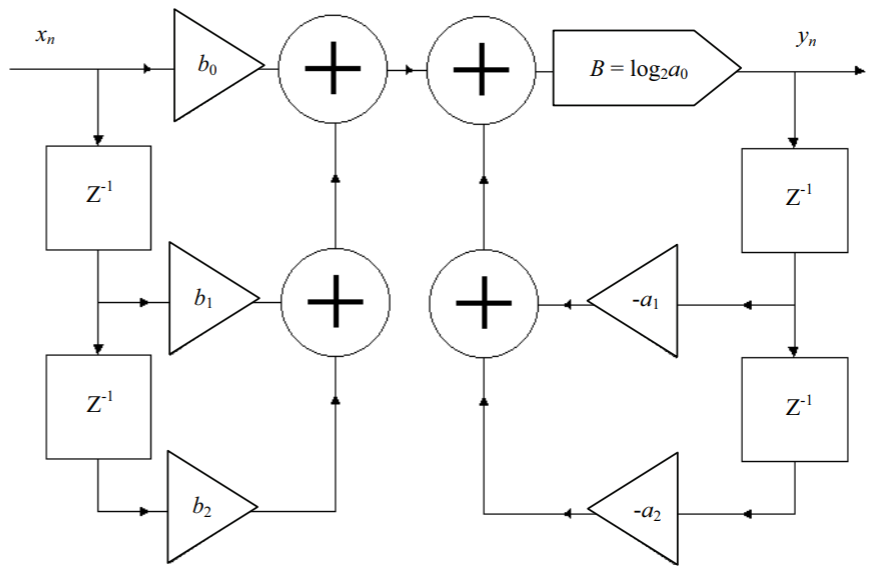
\includegraphics[width=\textwidth]{imgs/img1}
  \caption{Структура звена рекурсивного ЦНП-фильтра}
  \label{fig:figure1}
\end{figure}

Формально задача машинного синтеза рекурсивного фильтра описывается системой
\begin{gather}
\left\{\begin{aligned}
  &F^{o}\left(\boldsymbol{I X}^{\boldsymbol{o}}\right)=
    \min F(\boldsymbol{I X}),  \quad
      \boldsymbol{I X} \in I^{6 m},\\
  &-2^{R-1} \leq a_{d i} \leq 2^{R-1}-1, \quad \quad d=0,2, \quad i=1,\ldots,m\\
  &a_{0 i} \leq 2^{R-1}-1, \quad d=0,2, \quad \quad i=1,\ldots,m\\
  &a_{0 i} \in\left\{2^{q}\right\}, \quad \quad q=0,\ldots,R-1\\
  &\left(\left|b_{0 i}\right|+\left|b_{1 i}\right|+\left|b_{2 i}\right|+\left|a_{1 i}\right|+\left|a_{2 i}\right|\right)<2^{R-1}, \quad \quad i=1,\ldots,m
\end{aligned}\right.
\end{gather}
где $I^{6m}$ -- целочисленное пространство параметров фильтра, $m$ -- число звеньев второго порядка, $d$ -- индекс
коэффициента передаточной функции звена \eqref{eq:iir_cascad}.

Общая экстремальная задача синтеза записана относительно целочисленного пространства $I^{6m}$ параметров (коэффициентов фильтра). Поисковое итеративное решение экстремальной задачи ЦНП в заданном пространстве параметров осуществляет программный алгоритмический комплекс через
модельный блок программы для расчёта текущих функциональных характеристик фильтра. 

Вектор $\boldsymbol{I X}^{\boldsymbol{o}}$, минимизирующий скалярную
целевую функцию $F$, является эффективным решением задачи параметрического синтеза рекурсивного ЦНП-фильтра.

\subsection{Некурсивные фильтры}

В нерекурсивных ЦНП-фильтрах отклик фильтра  вычисляется через прямую линейную свёртку значений входной КИХ-последовательности $x_n$ 
\begin{equation}
  y_{n}=\sum_{k=0}^{N-1} \frac{b_{k}}{a_{0}} \cdot x_{n-k},
\end{equation}
поэтому такие фильтры всегда устойчивы и имеют конечную импульсную характеристику (finite impulse response -- FIR). Входное окно КИХ-фильтра составляет $N$ отсчётов, при этом значение $N$ определяет порядок нерекурсивного фильтра.

Передаточная функция каскадного соединения $m$-звеньев второго порядка нерекурсивного ЦНП-фильтра может быть записана так:
\begin{equation}
  H(z)=\prod_{i=1}^{m} \frac{b_{0 i}+b_{1 i} z^{-1}+b_{2 i} z^{-2}}{a_{0 i}}.
\end{equation}

Уравнение одного звена нерекурсивного фильтра имеет вид:
\begin{equation}
  y_{n}=\frac{b_{0} x_{n}+b_{1} x_{n-1}+b_{2} x_{n-2}}{a_0},
\end{equation}
где коэффициент $a_0$  во всех  $m$  звеньях также принадлежит биномиальному целочисленному ряду $a_{0 i}
\in\left\{2^{q}\right\}, q=\overline{0, R-1} \quad i=\overline{1, m}$. На рис. \ref{fig:figure2} приведена типичная
структура звеньев нерекурсивного цифрового фильтра.

\begin{figure}[H]
  \centering
  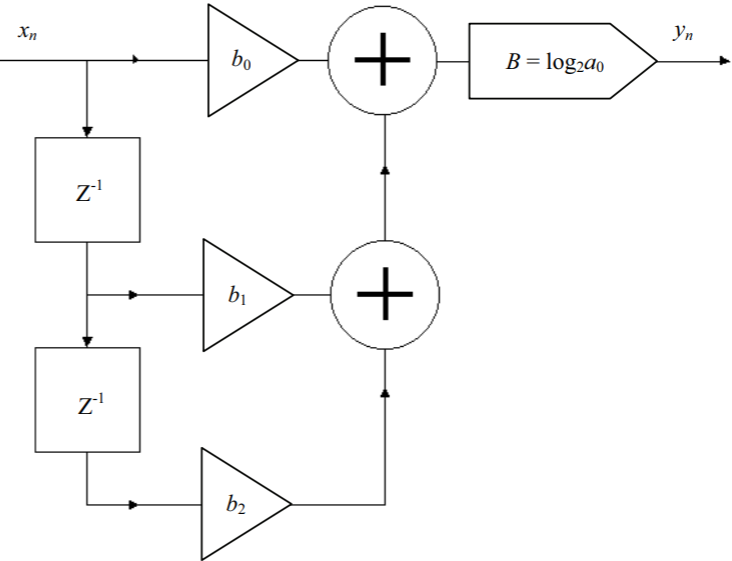
\includegraphics[width=\textwidth]{imgs/img2}
  \caption{Структура звена нерекурсивного ЦНП-фильтра}
  \label{fig:figure2}
\end{figure}

Постановка задачи целочисленного нелинейного программирования для машинного синтеза нерекурсивного фильтра выглядит следующим образом:

\begin{gather}
\left\{\begin{aligned}
  &F^{o}\left(\boldsymbol{I X}^{\boldsymbol{o}}\right)=
    \min F(\boldsymbol{I X}),  \quad
      \boldsymbol{I X} \in I^{4 m},\\
  &-2^{R-1} \leq b_{d i} \leq 2^{R-1}-1, \quad \quad d=0,2, \quad i=1,\ldots,m\\
  &a_{0 i} \in\left\{2^{q}\right\}, \quad \quad q=0,\ldots,R-1\\
  &\left(\left|b_{0 i}\right|+\left|b_{1 i}\right|+\left|b_{2 i}\right|\right)<2^{R-1}, \quad \quad i=1,\ldots,m
\end{aligned}\right.
\end{gather}
где $I^{4m}$ -- целочисленное пространство параметров фильтра, $m$ - число КИХ-звеньев второго
порядка, $d$ -- индекс коэффициента передаточной функции одного звена КИХ-фильтра, $R$ -- разрядность микропроцессора. 


\section{Лабораторная установка}

Для выполнения лабораторной работы используются три программных модуля: 
\begin{itemize}
  \item программа параметрического синтеза и анализа ЦНП-фильтров,
  \item среда программирования микроконтроллера IAR,
  \item панорамный измеритель частотных характеристик фильтра. 
\end{itemize}
\begin{figure}[H]
  \centering
  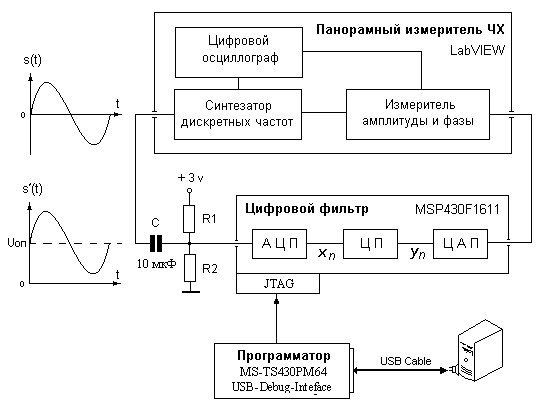
\includegraphics[width=\textwidth]{imgs/img3}
  \caption{Схема лабораторной установки}
  \label{fig:figure3}
\end{figure}

В лабораторную установку входят отладочная плата MSP-FET430UIF с микроконтроллером MSP430F1611, на котором реализован исследуемый ЦЦФ. Программирование микроконтроллера осуществляется с помощью программатора MSP-TS430PM64 через интерфейс JTAG. 

Измерение частотных характеристик фильтра осуществляется на реальном сигнале с помощью автоматизированной панорамной измерительной системы, разработанной в среде виртуальных приборов LabVIEW. Синтезатор частоты генерирует качественный гармонический сигнал амплитудой 0,5 вольта на дискретных частотах заданного пользователем интервала измерения от частоты $f_{\min}$ до частоты $f_{\max}$ с шагом $f_s$ (все частоты задаются в Гц). Сигнал с синтезатора частоты в положительной полярности подаётся на вход АЦП цифрового фильтра, а выходной сигнал ЦАП – на измеритель амплитуды и фазы. Время генерации входного гармонического сигнала -- 10 периодов на каждой дискретной частоте. Этого вполне достаточно для полного установления колебаний в исследуемой системе. В конце каждого интервала генерации производится измерение амплитуды и фазы выходного сигнала. 
  
Форма входного и выходного сигналов на каждой дискретной частоте отображается на панели цифрового осциллографа, входящего в состав панорамного измерителя частотных характеристик. После завершения измерений в заданном интервале частот производится построение графиков АЧХ и ФЧХ исследуемого фильтра. Эти графики могут быть распечатаны или сохранены в файле средствами LabVIEW.


\subsection{Программа синтеза и анализа цифровых фильтров}
Программа позволяет осуществлять параметрический синтез как рекурсивных (IIR), так и нерекурсивных (FIR) цифровых фильтров различного порядка в широкой области допустимых изменений целочисленных параметров (коэффициентов) фильтра, проводить подробный анализ полученного оптимального решения в частотной области, выводить на печать графики частотных характеристик синтезированного фильтра, а также формировать файл протокола решения текущей задачи синтеза. 
\begin{figure}[h!]
  \centering
  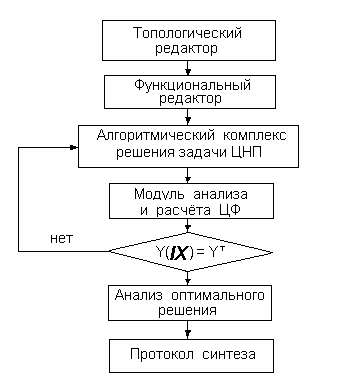
\includegraphics[width=0.6\textwidth]{imgs/img4}
  \caption{Блок-схема учебной программы синтеза}
  \label{fig:figure1}
\end{figure}
Рассмотрим взаимодействие основных модулей программы в контексте выполнения основных этапов решения конкретной задачи синтеза цифрового фильтра.

\textbf{На первом этапе} формируется типовой топологический файл задания на синтез  name.top, имя которого определяет пользователь. В данных файлах содержится описание структуры синтезируемого фильтра, определяются границы изменения его варьируемых коэффициентов и их начальное значения, указывается порядок и тип синтезируемого фильтра.

\textbf{На  втором этапе} необходимо осуществить ввод требуемых характеристик синтезируемого фильтра и сформировать целевую функцию. Для этого служит графический редактор функциональных характеристик (функциональный редактор), который необходимо вызвать из основного меню программы.

\textbf{На третьем этапе} программный алгоритмический комплекс осуществляет поисковое итеративное решение экстремальной задачи ЦНП-синтеза в заданном пространстве целочисленных варьируемых коэффициентов фильтра, обращаясь к модельному блоку программы для расчёта текущих функциональных характеристик фильтра по заданной его модели. Старт синтеза осуществляется нажатием соответствующей «горячей» кнопкой основного меню программы.

\textbf{На четвёртом этапе} осуществляется подробное исследование найденного эффективного решения задачи ЦНП-синтеза в модуле анализа пакета (кнопка основного меню «Анализ») с построением графиков всех характеристик цифрового фильтра, их распечаткой и формированием стандартного протокола решения задачи синтеза.

\subsection{Микроконтроллер и его программирование}

В данной лабораторной работе изучаются вопросы программной реализации синтезированного целочисленного фильтра на микропроцессорном контроллере, широко используемом в современной радиоэлектронике в качестве встроенного средства контроля, цифровой обработки или управления характеристиками различных объектов или процессов. 

На кристалле такого контроллера, кроме микропроцессора, находятся весь набор необходимых компонентов  вычислительного комплекса, таких как АЦП, системный контроллер, устройства постоянной и перепрограммируемой памяти, аппаратные умножители и сумматоры, ЦАП и др.

Реализация синтезированного ЦНП-фильтра сводится к программированию микроконтроллера, т.е. занесению в ПЗУ найденных целочисленных коэффициентов фильтра и программы их обработки –- расчёта выходного отклика фильтра по его линейно-разностному уравнению  для рекурсивного фильтра либо по прямой свёртке для нерекурсивного.

Программирование микроконтроллера ведётся в среде IAR Emb\-edd\-ed Wo\-rkbe\-nch for MSP430 на языке С++. 
В состав среды программирования входят компилятор, редактор с подсветкой синтаксиса, менеджер проектов, инструментальные средства отладки. Компилятор, входящий в пакет, представляет собой узкоспециализированный компилятор C, который генерирует код на ассемблере TI/IAR MSP430. Загрузка программы в память контроллера осуществляется с помощью встроенного в эту среду FET-Debugger, использующего интерфейс JTAG.
\newpage


\section{Синтез цифровых целочисленных фильтров}
\subsection{Полосовые фильтры}
\begin{figure}[H]
  \centering
  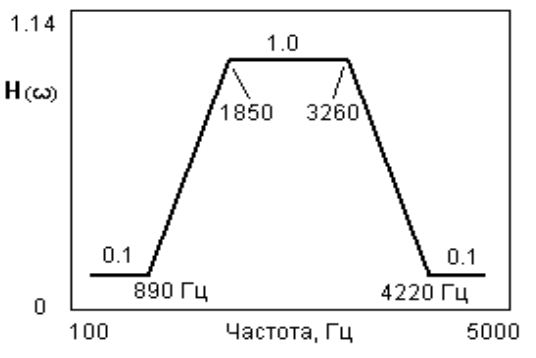
\includegraphics[width=0.6\textwidth]{imgs/img6.png}
  \caption{Требуемая АЧХ полосового фильтра}
  \label{fig:}
\end{figure}
\subsubsection{Полосовой FIR-фильтр}
\begin{figure}[H]
  \centering
  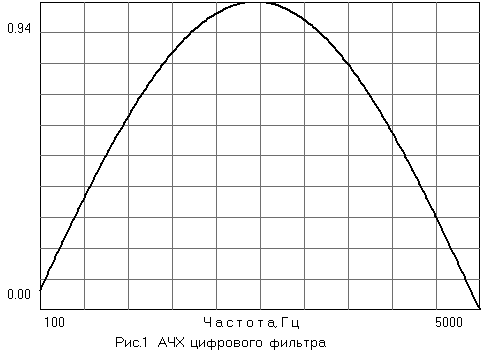
\includegraphics[width=0.7\textwidth]{data/Z1_PPF/gain_FIR_2P.png}
  \caption{АЧХ полосового FIR-фильтра второго порядка, СКО=0.137}
  \label{fig:FIR_2p}
\end{figure}
\begin{figure}[H]
  \centering
  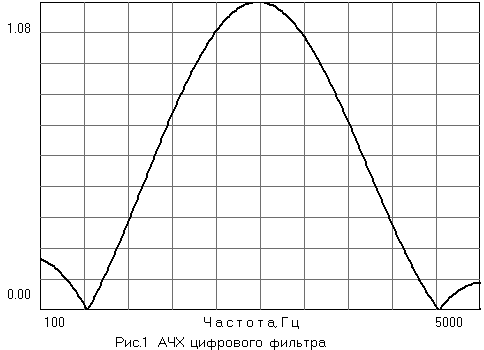
\includegraphics[width=0.7\textwidth]{data/Z1_PPF/gain_FIR_4P.png}
  \caption{АЧХ полосового FIR-фильтра четвёртого порядка, СКО=0.048}
  \label{fig:FIR_4p}
\end{figure}
\subsubsection{Полосовой IIR-фильтр}
\begin{figure}[H]
  \centering
  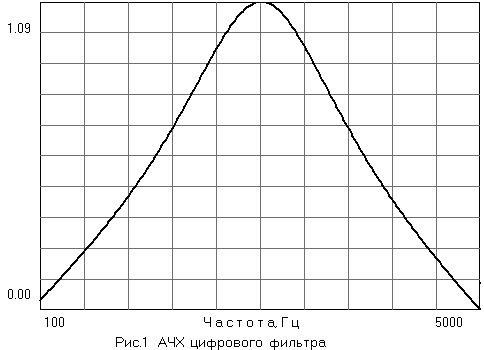
\includegraphics[width=0.7\textwidth]{data/Z1_PPF/gain_IIR2P.png}
  \caption{АЧХ полосового IIR-фильтра второго порядка, СКО=0.084}
  \label{fig:IIR_2p}
\end{figure}
\begin{figure}[H]
  \centering
  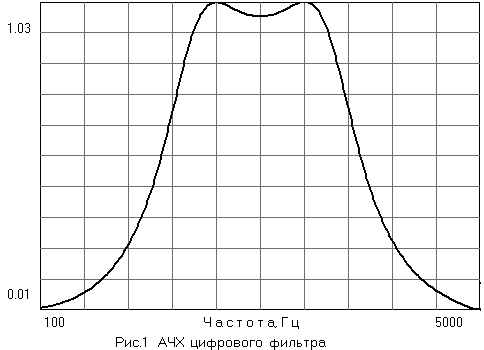
\includegraphics[width=0.7\textwidth]{data/Z1_PPF/gain_IIR4P.png}
  \caption{АЧХ полосового IIR-фильтра четвёртого порядка, СКО=0.013}
  \label{fig:IIR_4p}
\end{figure}



\begin{figure}[H]
  \centering
  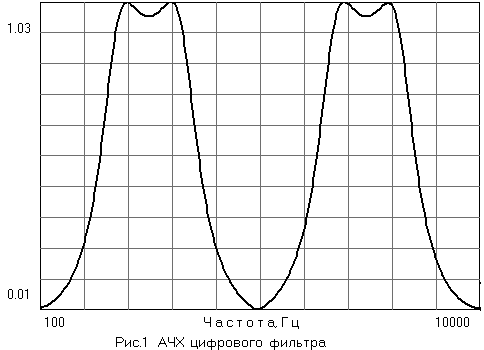
\includegraphics[width=0.7\textwidth]{data/Z1_PPF/gain_IIR4P_FD.png}
  \caption{АЧХ полосового IIR-фильтра четвёртого порядка, $f_{\max}=f_d$}
  \label{fig:}
\end{figure}
\begin{figure}[H]
  \centering
  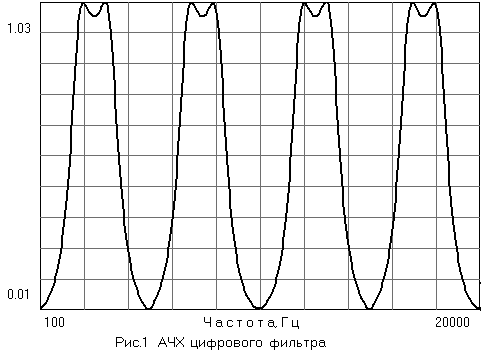
\includegraphics[width=0.7\textwidth]{data/Z1_PPF/gain_IIR4P_2FD.png}
  \caption{АЧХ полосового IIR-фильтра четвёртого порядка, $f_{\max}=2f_d$}
  \label{fig:}
\end{figure}
\begin{figure}[H]
  \centering
  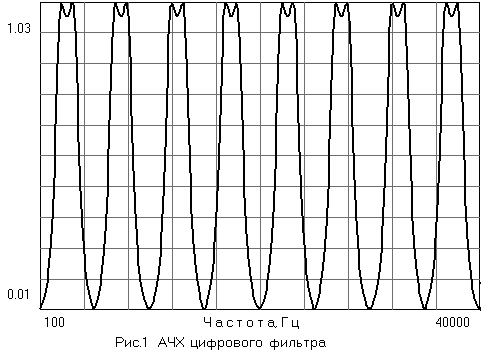
\includegraphics[width=0.7\textwidth]{data/Z1_PPF/gain_IIR4P_4FD.png}
  \caption{АЧХ полосового IIR-фильтра четвёртого порядка, $f_{\max}=4f_d$}
  \label{fig:}
\end{figure}

\begin{figure}[H]
  \centering
  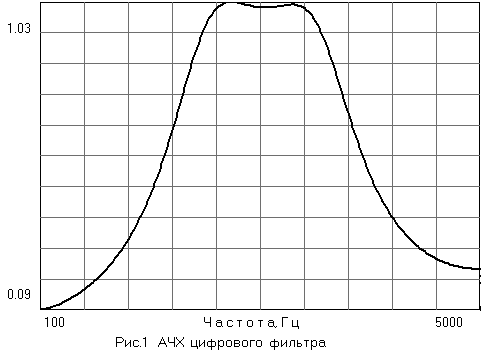
\includegraphics[width=0.7\textwidth]{data/Z1_PPF/gain_IIR_4p_R4.png}
  \caption{АЧХ полосового IIR-фильтра четвёртого порядка, $R=4$ СКО=0.058}
  \label{fig:}
\end{figure}
\begin{figure}[H]
  \centering
  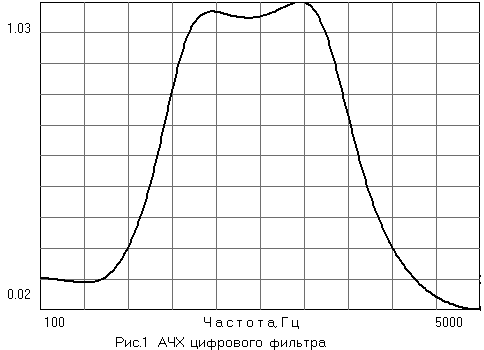
\includegraphics[width=0.7\textwidth]{data/Z1_PPF/gain_IIR_4p_R8.png}
  \caption{АЧХ полосового IIR-фильтра четвёртого порядка, $R=8$ СКО=0.026}
  \label{fig:}
\end{figure}
\begin{figure}[H]
  \centering
  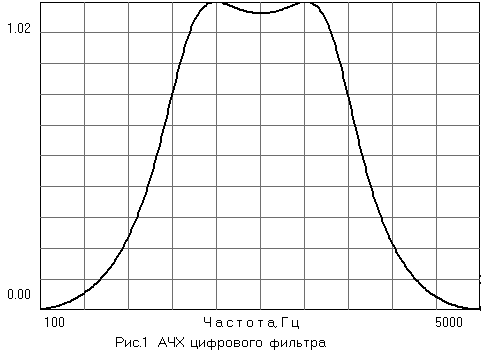
\includegraphics[width=0.7\textwidth]{data/Z1_PPF/gain_IIR_4p_R16.png}
  \caption{АЧХ полосового IIR-фильтра четвёртого порядка, $R=16$ СКО=0.011}
  \label{fig:}
\end{figure}

\begin{table}[H]
\centering
\caption{Оптимальные  коэффициенты  полосового  рекурсивного  фильтра  четвёртого порядка}
\vspace{0.5em}
\begin{tabular}{|c|c|c|c|c|c|c|}
\hline
Номер звена & $a_0$ & $a_1$ & $a_2$ & $b_0$ & $b_1$ & $b_2$ \\ \hline
1           & 8192    & 5999    & 4553    & 2758   & 931     & -2014    \\ \hline
2           & 8192    & -5237   & 4571    & 5840   & -1869   & -2956    \\ \hline
\end{tabular}
\end{table}
По результатам анализа синтеза фильтров сделали вывод о том, что селективные свойства цифровых фильтров увеличиваются:
\begin{enumerate}
  \vspace{-0.6em}
  \item при переходе от нерекурсивных фильтров к рекурсивным;\\[-1.8em]
  \item с увеличением порядка;\\[-1.8em]
  \item с увеличением разрядности.\\[-1.8em]
\end{enumerate}

Частотные характеристики фильтра являются непрерывными, периодическими функциями и наблюдается чётная симметрия АЧХ относительно частоты Найквиста.

\subsection{Гауссов фильтр}
% Нормированная резонансная характеристика для гауссовой кривой определяется как
% \begin{equation}
%   y(\xi)=e^{-\frac{\xi^{2}}{\alpha}},
% \end{equation}
% где  $\xi=f-f_0$ -- абсолютная расстройка от резонансной частоты, а параметр $\alpha$  определяет нормированную полосу пропускания гауссовой кривой:
% \begin{equation}
%   \alpha=\frac{\Pi^{2}}{4 \ln \sqrt{2}}
% \end{equation}
% здесь $\Pi$ -- абсолютная полоса пропускания по уровню 0.7. 
\subsubsection{Гауссов FIR-фильтр}
\begin{figure}[H]
  \centering
  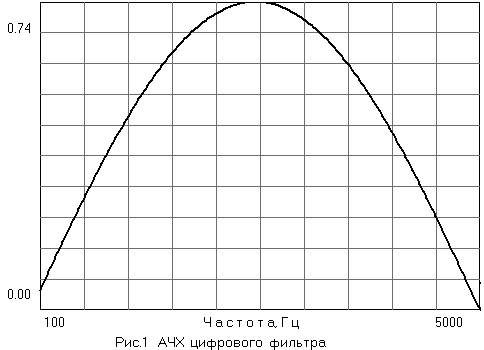
\includegraphics[width=0.7\textwidth]{data/Z1_GAUSS/gain_FIR_2p.png}
  \caption{АЧХ гауссова FIR-фильтра второго порядка, СКО=0.209}
  \label{fig:}
\end{figure}
\begin{figure}[H]
  \centering
  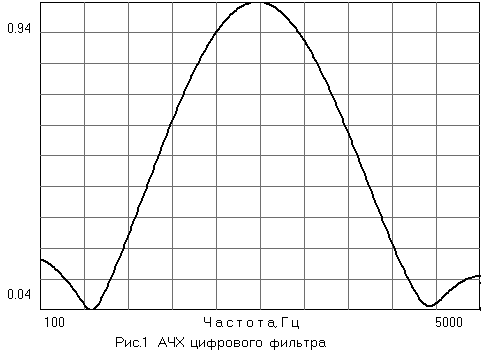
\includegraphics[width=0.7\textwidth]{data/Z1_GAUSS/gain_FIR_4p.png}
  \caption{АЧХ гауссова FIR-фильтра четвёртого порядка, СКО=0.093}
  \label{fig:}
\end{figure}
\subsubsection{Гауссов IIR-фильтр}
\begin{figure}[H]
  \centering
  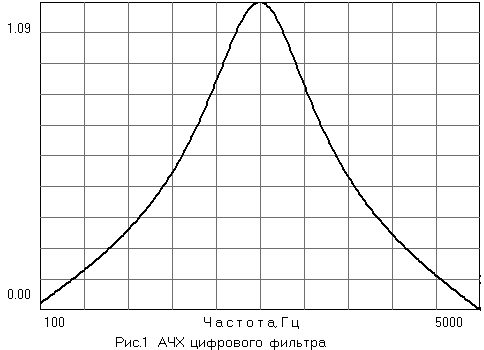
\includegraphics[width=0.7\textwidth]{data/Z1_GAUSS/gain_IIR_2p.png}
  \caption{АЧХ гауссова IIR-фильтра второго порядка, СКО=0.055}
  \label{fig:}
\end{figure}
\begin{figure}[H]
  \centering
  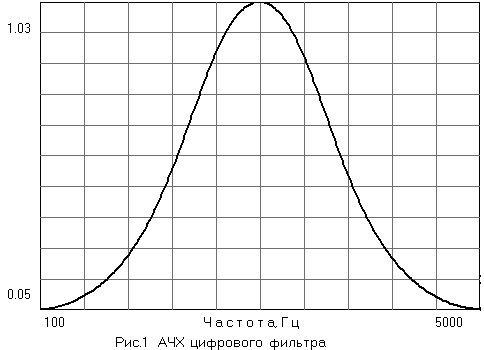
\includegraphics[width=0.7\textwidth]{data/Z1_GAUSS/gain_IIR_4p.png}
  \caption{АЧХ гауссова IIR-фильтра четвёртого порядка, СКО=0.007}
  \label{fig:}
\end{figure}




\begin{figure}[H]
  \centering
  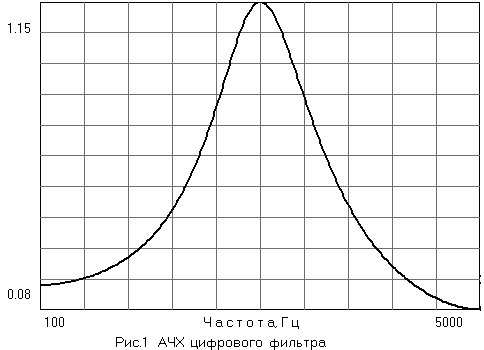
\includegraphics[width=0.7\textwidth]{data/Z1_GAUSS/gain_IIR_4p_R4.png}
  \caption{АЧХ гауссова IIR-фильтра четвёртого порядка, $R=4$ СКО=0.047}
  \label{fig:}
\end{figure}
\begin{figure}[H]
  \centering
  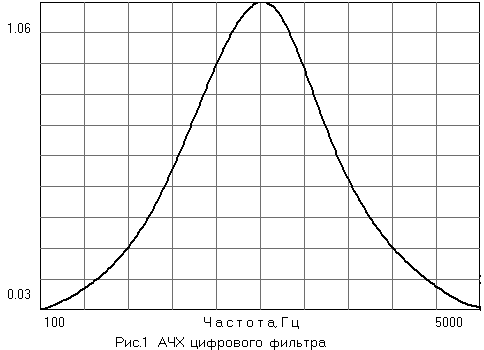
\includegraphics[width=0.7\textwidth]{data/Z1_GAUSS/gain_IIR_4p_R8.png}
  \caption{АЧХ гауссова IIR-фильтра четвёртого порядка, $R=8$ СКО=0.017}
  \label{fig:}
\end{figure}
\begin{figure}[H]
  \centering
  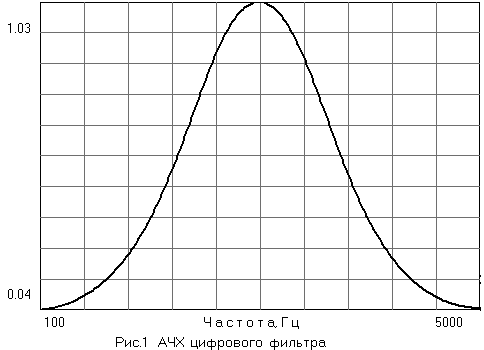
\includegraphics[width=0.7\textwidth]{data/Z1_GAUSS/gain_IIR_4p_R16.png}
  \caption{АЧХ гауссова IIR-фильтра четвёртого порядка, $R=16$ СКО=0.009}
  \label{fig:}
\end{figure}

Для IIR-фильтра 4-го порядка ($R=16$) были определены по АЧХ центральная частота $f_0$, полоса пропускания $\Pi$, добротность $Q$ и коэффициент прямоугольности $\zeta$:
\begin{gather}
  f_0=2500 \text{ Гц}, \quad
  \Pi=2\Delta f_{0.7} =1559.4 \text{ Гц}, \quad
  Q=\frac{f_0}{2\Delta f_{0.7}}=2.06, \\
  \text{КП}=\frac{2\Delta f_{0.7}}{2\Delta f_{0.1}}=0.36 \text{ Гц}
\end{gather}

% \subsection{IIR-фильтры}

\begin{table}[H]
\centering
\caption{Оптимальные  коэффициенты  гауссова  рекурсивного  фильтра  четвёртого порядка}
\vspace{0.5em}
\begin{tabular}{|c|c|c|c|c|c|c|}
\hline
Номер звена & $a_0$ & $a_1$ & $a_2$ & $b_0$ & $b_1$ & $b_2$ \\ \hline
1           & 8192    & -2909   & 3405    & 4170    & 8675    & 3833    \\ \hline
2           & 16384   & 5793    & 7153    & -5020   & 6826    & -2695   \\ \hline
\end{tabular}
\end{table}

В этом задании было получено, что селективные свойства фильтра увеличиваются при переходе от нерекурсивного фильтра к рекурсивному, при увеличении порядка и разрядности. Для исследованных фильтров частотная характеристика - периодическая и непрерывная функция, симметричная относительно частоты Найквиста. 




\newpage
\section{Исследование цифрового тракта}

С помощью встроенного в панорамный измеритель осциллографа была зафиксирована форма
входного и выходного (с ЦАП) сигналов на частотах $f_{\max}$=200, 500 и 1000 Гц ($f_{\min}$=10 Гц, шаг $f_s$=20 Гц):

\begin{figure}[H]
  \centering
  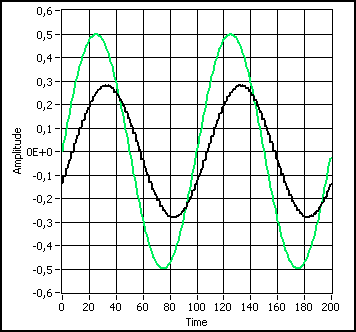
\includegraphics[width=0.5\textwidth]{data/Z4_FN4/signal_200.png}
  \caption{$f_{\max}$=200 Гц}
  \label{fig:}
\end{figure}
\begin{figure}[H]
  \centering
  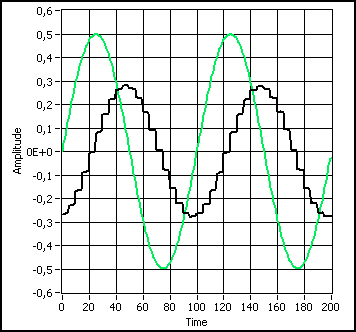
\includegraphics[width=0.5\textwidth]{data/Z4_FN4/signal_500.png}
  \caption{$f_{\max}$=500 Гц}
  \label{fig:}
\end{figure}
\begin{figure}[H]
  \centering
  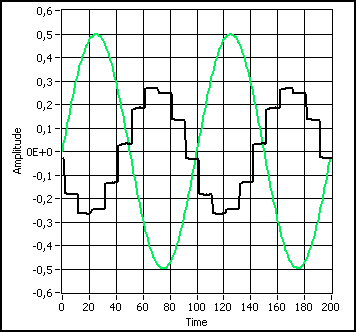
\includegraphics[width=0.5\textwidth]{data/Z4_FN4/signal_1000.png}
  \caption{$f_{\max}$=1000 Гц}
  \label{fig:}
\end{figure}

При приближении к частоте Найквиста форма сигнала становится более ступенчатой. Форма выходного сигнала отражает процесс дискретизации и квантования при обработке сигнала: количество ступенек в сигнале равно количеству выборок аналогового сигнала $N$, которое определяется по формуле
\begin{equation}
  N=\frac{f_d}{f_s}
\end{equation}
Где $f_d$ -- частота дискретизации сигнала, а $f_s$ -- частота сигнала на входе приемника.

\section{Синтез IIR-ФНЧ с линейной фазой}
\begin{figure}[H]
  \centering
  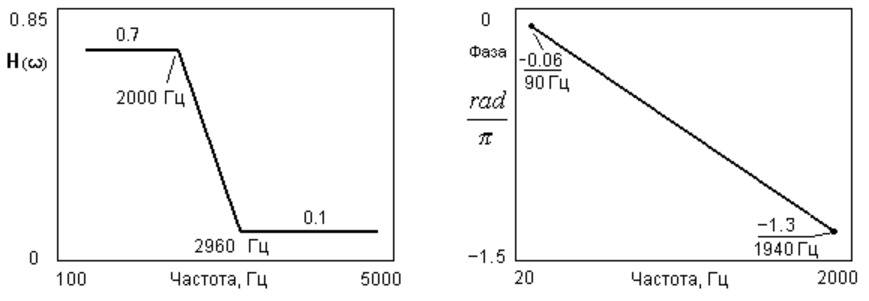
\includegraphics[width=\textwidth]{imgs/img5.png}
  \caption{Требуемые АЧХ и ФЧХ}
  \label{fig:}
\end{figure}

\begin{figure}[H]
  \centering
  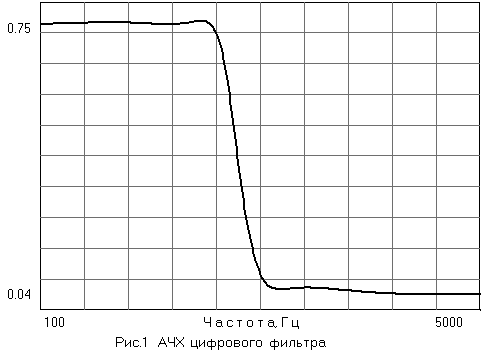
\includegraphics[width=0.7\textwidth]{data/Z4_FN4/Gain(0).png}
  \caption{АЧХ при синтезе без учета фазовых требований ($\beta_2=0$) СКО=0.003}
  \label{fig:}
\end{figure}
\begin{figure}[H]
  \centering
  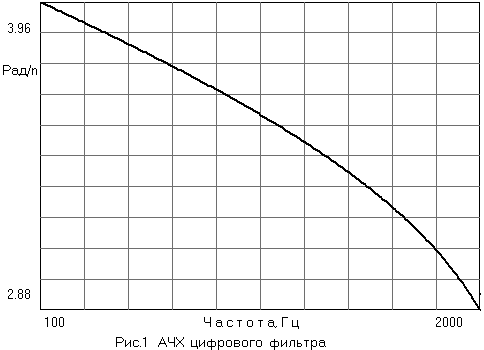
\includegraphics[width=0.7\textwidth]{data/Z4_FN4/Faza(0).png}
  \caption{ФЧХ при синтезе без учета фазовых требований ($\beta_2=0$) СКО=15.23, max err=21.67}
  \label{fig:}
\end{figure}
\begin{figure}[H]
  \centering
  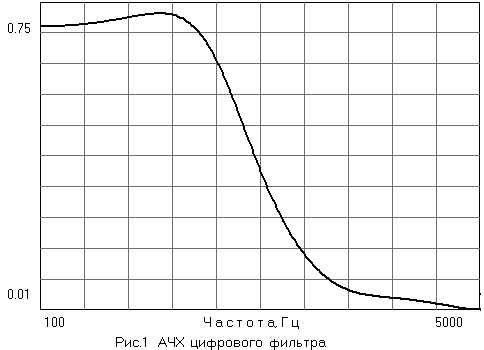
\includegraphics[width=0.7\textwidth]{data/Z4_FN4/Gain(4).png}
  \caption{АЧХ при синтезе с учетом фазовых требований ($\beta_2=4$) СКО=0.012}
  \label{fig:}
\end{figure}
\begin{figure}[H]
  \centering
  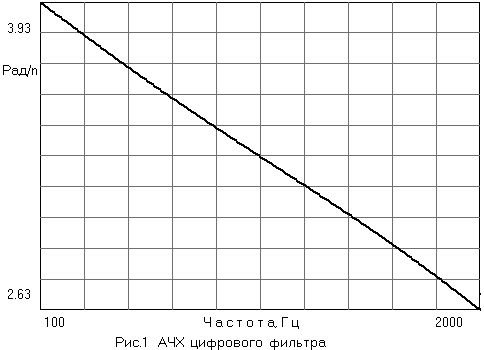
\includegraphics[width=0.7\textwidth]{data/Z4_FN4/Faza(4).png}
  \caption{ФЧХ при синтезе с учетом фазовых требований ($\beta_2=4$) НЧХ=0.017}
  \label{fig:}
\end{figure}

Из протокола синтеза в программу расчёта отклика были введены оптимальные коэффициенты синтезированного фильтра с учетом фазовых требований и осуществлены трансляция и загрузка программы в микроконтроллер. С помощью панорамного измерителя  измерены АЧХ и ФЧХ синтезированного фильтра:

\begin{figure}[H]
  \centering
  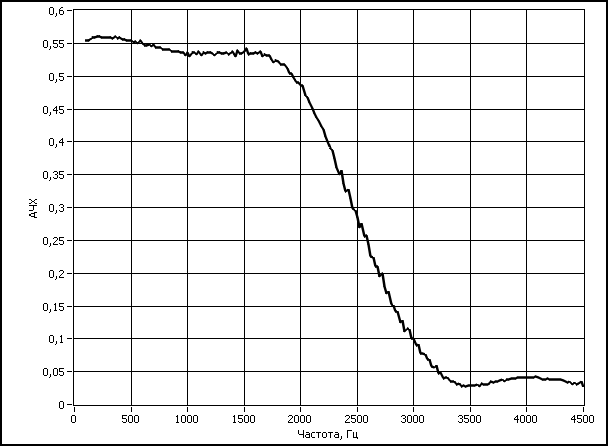
\includegraphics[width=0.7\textwidth]{data/Z4_FN4/Gain(4)_Pan.png}
  \caption{АЧХ с панорамного измерителя}
  \label{fig:}
\end{figure}

\begin{figure}[H]
  \centering
  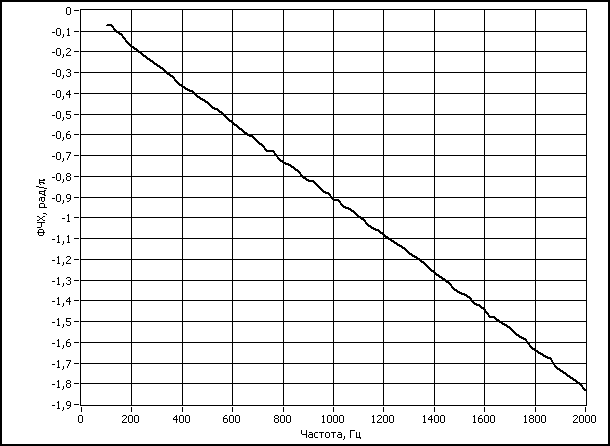
\includegraphics[width=0.7\textwidth]{data/Z4_FN4/Faza(4)_Pan_Faza.png}
  \caption{ФЧХ с панорамного измерителя}
  \label{fig:}
\end{figure}

При синтезе без учета фазовых требований СКО составляет 0.003, а нелинейность ФЧХ $15^\circ$. При синтезе с учётом фазовых требований селективность ухудшается (СКО=0.012), но фазовые искажения уменьшаются до $2.7^\circ$. Это объясняется тем, что модуль и фаза коэффициента передачи связаны преобразованием Гильберта.




\addcontentsline{toc}{section}{Заключение}
\section*{Заключение}

В процессе выполнения работы были синтезированы рекурсивные и не рекурсивные модельные  ЦНП-фильтры и фильтры на микроконтроллере, оценены селективные свойства и рекомендуемый рабочий диапазон реализованного цифрового фильтра нижних частот.

Синтезирование рекурсивного фильтра проводилось с учетом и без учета фазовых требований. Если не учитывать фазовые требования, АЧХ практически совпадает с требуемой, однако появляется нелинейность ФЧХ в полосе пропускания. 

При синтезе ФНЧ с учетом фазовых требований, селективность фильтра ухудшилась (СКО=2.776), а фазовые искажения существенно уменьшились.




\end{document}
